\documentclass{beamer}

\mode<presentation> {
  \usetheme{CambridgeUS}
  \setbeamertemplate{footline}[page number]
  \setbeamertemplate{navigation symbols}{}
}

\usepackage{listings}
\usepackage{graphicx}
\usepackage{tikz}
\usepackage{booktabs} % Allows the use of \toprule, \midrule and \bottomrule in tables

\lstdefinestyle{erlang}{
   language        = erlang,
   showstringspaces= false,
   breaklines      = true,
   keywordstyle    = {\bfseries},
   keywordstyle    = [2]{\color{green}},
   keywordstyle    = [3]{\color{red}},
   alsoletter      = {?, :},
   morekeywords    = {
     fun,
     begin},
   morekeywords    = [2]{
     ?FORALL,
     ?LET},
   morekeywords    = [3]{
     eqc:numtests,
     eqc:quickcheck,
     eqc_c:start,
     eqc\_statem:show\_states,
     car,
     car\_xml}
}
\lstdefinestyle{c}{
  language        = c,
  commentstyle    = \color{purple},
  keywordstyle    = \color{violet},
  showstringspaces= false
}
\lstdefinestyle{autosar}{
  breaklines      = false,
  frame           = l,
  showstringspaces= false,
  string          = [s]{``}{''},
  morestring      = [b]",
  basicstyle      = \color{red},
  keywordstyle    = \color{blue},
  commentstyle    = \color{green},
  stringstyle     = \color{green},
  moredelim       = [is][\color{cyan}]{|}{|},
  literate        = {<=}{{$\leq$}}{1} %% observe no comma
                    {>=}{{$\geq$}}{1},
  identifierstyle = \color{black},
  emph            = {
    WdgMExpiredSupervisionCycleTol,
    WdgM_MainFunction,
    WdgM_SetMode,
    WdgM_Init,
    WdgM_DeInit,
    WdgM_CheckpointReached,
    WdgM_CalculateAliveSupervision,
    WdgM_CheckLogicalSupervisedEntities
  },
  emphstyle       = {\color{cyan}},
  morekeywords    = {
    WDGM\_CORRECT,
    WDGM\_INCORRECT,
    WDGM\_GLOBAL\_STATUS\_OK,
    WDGM\_GLOBAL\_STATUS\_FAILED,
    WDGM\_GLOBAL\_STATUS\_EXPIRED,
    WDGM\_GLOBAL\_STATUS\_STOPPED,
    WDGM\_GLOBAL\_STATUS\_DEACTIVATED,
    WDGM\_LOCAL\_STATUS\_OK,
    WDGM\_LOCAL\_STATUS\_FAILED,
    WDGM\_LOCAL\_STATUS\_EXPIRED,
    WDGM\_LOCAL\_STATUS\_DEACTIVATED
  }
}
\lstset{language=c, mathescape}


%------------------------------------------------
% TITLE PAGE
%------------------------------------------------

\title{Evaluation of validity of verification methods}

\author{Oskar Ingemarsson, Sebastian Weddmark Olsson}
\institute{Chalmers University of Technology, Mecel AB}
\date{\today}

\begin{document}

\begin{frame}
  \titlepage
\end{frame}

\begin{frame}
  \frametitle{Overview}
  \tableofcontents
\end{frame}

%------------------------------------------------
% PRESENTATION SLIDES
%------------------------------------------------
%================================================
\section{Introduction}
%================================================
\begin{frame}[fragile]
  \frametitle{Introduction}
  \begin{block}{Background}
    \begin{itemize}
        \item Circa 80 control units
        \item Close to hundred million lines of code
        \item Vehicles become more and more complex
        \item More functionality
        \item Safety critical
        \item Testing more then half the production cost
    \end{itemize}
   \end{block}
\end{frame}

\begin{frame}<1>[label=glossary]
  \frametitle{Glossary}
  \begin{description}
    \item<1->[AUTOSAR (AUTomotive Open System ARchitecture)]
    \item<2->[Functional Safety (according to ISO~26262)]
    \item<3->[ASIL (Automotive Safety Integrity Level)]
    % \item<4->[WdgM (Wathdog Mangager)]
    \item<4->[Supervised entity]
    \item<5->[QuickCheck (A commercial testing tool)]
    %\item<2->
    %\item<2->[Checkpoint]
    %\item<3->[Mode]
%    \item[-]
  \end{description}
\end{frame}

\againframe<2>{glossary}
\againframe<3>{glossary}

\begin{frame}[fragile]
  \frametitle{Introduction}
  \begin{block}{Objective}
    \begin{itemize}
        \item Automation of tests on modules in AUTOSAR
        \item Examine if it is possible to reach the requirements for
          a higher ASIL classification, thus fulfilling more
          requirements within the concept of functional safety.
        % \item Functional Safety
    \end{itemize}
   \end{block}
  % \begin{block}{Resources}
  %   \begin{itemize}
  %       \item Model based testing
  %       \item QuickCheck
  %       \item Other
  %   \end{itemize}
  % \end{block}
\end{frame}


%================================================
\section{Watchdog Manager}
%================================================

\begin{frame}
  \frametitle{Watchdog Manager}
  \begin{block}{AUTOSAR specification}
    ``The Watchdog Manager supervises the execution of a configurable
    number of so called Supervised Entities. When it detects a violation
    of the configured temporal and/or logical constraints on program
    execution, it takes a number of configurable actions to recover from
    this failure.''
  \end{block}
\end{frame}

\againframe<4>{glossary}

\begin{frame}[fragile]
  \frametitle{Functions}
  \begin{block}{Getters}
    \begin{itemize}
      \item \lstinline!GetVersionInfo(VersionInfoType*)!
      \item \lstinline!GetMode(ModeType*)!
      \item \lstinline!GetLocalStatus(SupervisedEntityIdType, LocalStatusType*)!
      \item \lstinline!GetGlobalStatus(GlobalStatusType*)!
      \item \lstinline!GetFirstExpiredSEID(SupervisedEntityIdType*)!
    \end{itemize}
  \end{block}

  \begin{block}{Setters (interesting)}
    \begin{itemize}
      \item \lstinline!Init(ConfigType*)!
      \item \lstinline!DeInit()!
      \item \lstinline!PerformReset()!
      \item \lstinline!SetMode(ModeType, uint16)!
      \item \lstinline!MainFunction()!
      \item \lstinline!Checkpointreached(SupervisedEntityIdType, CheckpointIdType)!
    \end{itemize}
  \end{block}
\end{frame}

\begin{frame}
  \frametitle{Supervision mechanisms}
  \begin{itemize}
    \item Alive supervision
    \item Deadline supervision
    \item Logical supervision
  \end{itemize}
\end{frame}

%----------------------------------------------
% \subsection{Supervision algorithms}
%----------------------------------------------
%------------------------------------------------
% \subsection{Alive supervision}
%------------------------------------------------
% \begin{frame}
%   \frametitle{Alive Supervision}
%   \begin{block}{Statement}
%     A checkpoint that is monitored by alive supervision, should be
%     reached a number of times between each cycle.
%   \end{block}
% \end{frame}

% \begin{frame}
%   \frametitle{Alive Supervision}
%   \begin{block}{Values/Variables}
%     \begin{description}
%       \item[Expected alive indications] (EAI), property of mode, fixed
%         value from configuration
%       \item[Supervision reference cycle] (SRC), property of mode, fixed value
%         from configuration
%       \item[Min margin] (Min), property of mode, fixed value from configuration
%       \item[Max margin] (Max), property of mode, fixed value from configuration
%       \item[Alive counter] (AC)
%       \item[Supervision cycle] (SC)
%     \end{description}
%   \end{block}
% \end{frame}

% \begin{frame}[fragile]
%   \frametitle{Alive Supervision}
%   \begin{block}{The algorithm}
%     \begin{lstlisting}
%       if (SC Mod SRC == 0)
%         if (-Min $\in$ AI - EAI $\in$ Max)
%            Alive supervision is correct
%         else
%            Alive supervision is incorrect
%     \end{lstlisting}
%   \end{block}
%   Performed in the MainFunction, also increments the supervision
%   cycles.\\
%   CheckpointReached increments the alive indications for the
%   checkpoint.
% \end{frame}

% %------------------------------------------------
% % \subsection{Deadline supervision}
% %------------------------------------------------
% \begin{frame}
%   \frametitle{Deadline Supervision}
%   \begin{block}{Statement}
%     Deadline supervision checks that the time it takes between two
%     checkpoints is within a marginal
%   \end{block}
% \end{frame}

% \begin{frame}
%   \frametitle{Deadline Supervision}
%   \begin{block}{Values/Variables}
%     \begin{description}
%       \item[Start checkpoint] described by the configuration
%       \item[Stop checkpoint] described by the configuration
%       \item[Current timestamp]
%       \item[Min margin] fixed value from configuration
%       \item[Max margin] fixed value from configuration
%     \end{description}
%   \end{block}
% \end{frame}

% \begin{frame}[fragile]
%   \frametitle{Deadline Supervision}
%   \begin{block}{The algorithm}
%     \begin{lstlisting}
%     if( Start && Current == 0 )
%       // start the clock
%       Current = now()
%     else if( End && Min $\leq$ now() - Current $\leq$ Max )
%       Deadline supervision is correct
%     else
%       Deadline supervision is incorrect
%     \end{lstlisting}
%   \end{block}
%   Performed by CheckpointReached.
% \end{frame}

% %------------------------------------------------
% % \subsection{Logical supervision}
% %------------------------------------------------
% \begin{frame}
%   \frametitle{Logical Supervision}
%   \begin{block}{Statement}
%     The program that is supervised by logical supervision should have
%     a specific execution flow. The flow can be visualized by a
%     graph.
%   \end{block}
% \end{frame}

% \begin{frame}
%   \frametitle{Logical Supervision}
%   \begin{block}{Values/Variables}
%     \begin{description}
%       \item[Start checkpoints]
%       \item[End checkpoints]
%       \item[Transitions] between checkpoints
%       \item[Is started?] if the graph has been started
%       \item[Current checkpoint]
%     \end{description}
%   \end{block}
% \end{frame}

% \begin{frame}[fragile]
%   \frametitle{Logical Supervision}
%   \begin{block}{The algorithm}
%     \begin{lstlisting}
%       if( !Started && CP $\in$ Start checkpoints )
%         Started = true
%         Current = CP
%       else if( Started )
%         if( CP $\in$ End checkpoints )
%           Started = false
%           Current = null
%         // Causal ordered
%         else if( Current -> CP in Transitions )
%           Current = CP
%       else
%         Logical supervision is incorrect
%     \end{lstlisting}
%   \end{block}
%   Performed by CheckpointReached.
% \end{frame}

%------------------------------------------------
\subsection{The state machine}
%------------------------------------------------

\begin{frame}
  \frametitle{The state machine}
  \begin{description}
    \item[Global status] (for the watchdog manager)
    \item[Local status] (per supervised entity)
  \end{description}
  % Each supervised entity has a local supervision status that the main
  % function changes depending on the results from the local supervision
  % functions.\\

  % The global status of the watchdog manager is calculated after the
  % local supervision status for all supervised entities.\\

  % The new global status also depends on which global status the
  % watchdog manager had before.
\end{frame}

\begin{frame}
  \frametitle{The state machine}
  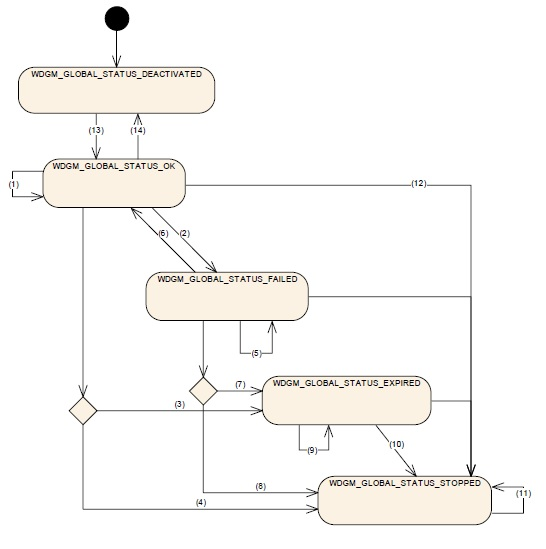
\includegraphics[keepaspectratio, width=0.7\linewidth]{globalstatuses}
\end{frame}

%================================================
\section{Implementation}
%================================================
%------------------------------------------------
\subsection{C code and QuickCheck}
%------------------------------------------------
\begin{frame}
  \frametitle{Generating the C byte code}
  \begin{tikzpicture}
\node at (4,4) {Configuration};
\draw[->] (4,3.8) -- (4,2);
\draw (3,0) rectangle (5,2) node at (4,1) {Generator};
\draw[->] (5,1) -- (9,1); %% -> Compiler
\node at (7,0.5) {Generated C code};
\node at (10,4) {C code}; %% -> Compiler
\draw[->] (10,3.8) -- (10,2);
\node at (10,-2) {Stubs/};
\node at (10,-2.5) {Dependencies};
\draw[->] (10,-1.8) -- (10,0);
\draw (9,0) rectangle (11,2) node at (10,1) {Compiler};
\draw[->] (11,1) -- (12,1);
\node at (13,1) {Byte code};
\end{tikzpicture}

\end{frame}

\againframe<5>{glossary}

% \begin{frame}
%   \frametitle{QuickCheck}
%   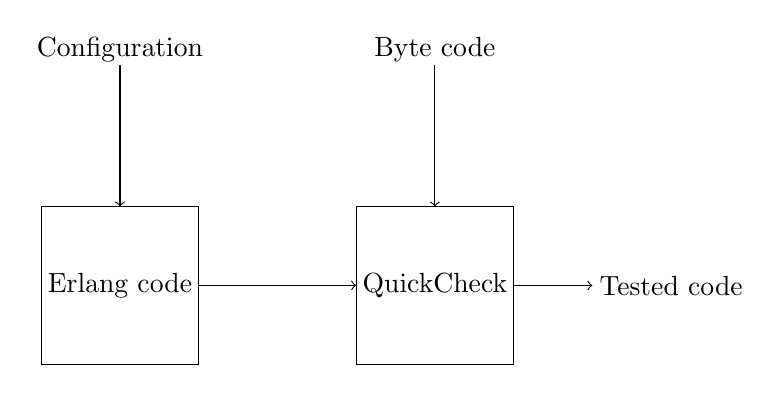
\begin{tikzpicture}
\node at (4,4) {Configuration};
\draw[->] (4,3.8) -- (4,2);
\draw (3,0) rectangle (5,2) node at (4,1) {Erlang code};
\draw[->] (5,1) -- (7,1); %% -> Compiler
\node at (8,4) {Byte code};
\draw[->] (8,3.8) -- (8,2);
\draw (7,0) rectangle (9,2) node at (8,1) {QuickCheck};
\draw[->] (9,1) -- (10,1);
\node at (11,1) {Tested code};
\end{tikzpicture}

% \end{frame}

%------------------------------------------------
% \subsection{Erlang implementation of AUTOSAR}
%------------------------------------------------

\begin{frame}
  \frametitle{How QuickCheck works}
  \centerline{
    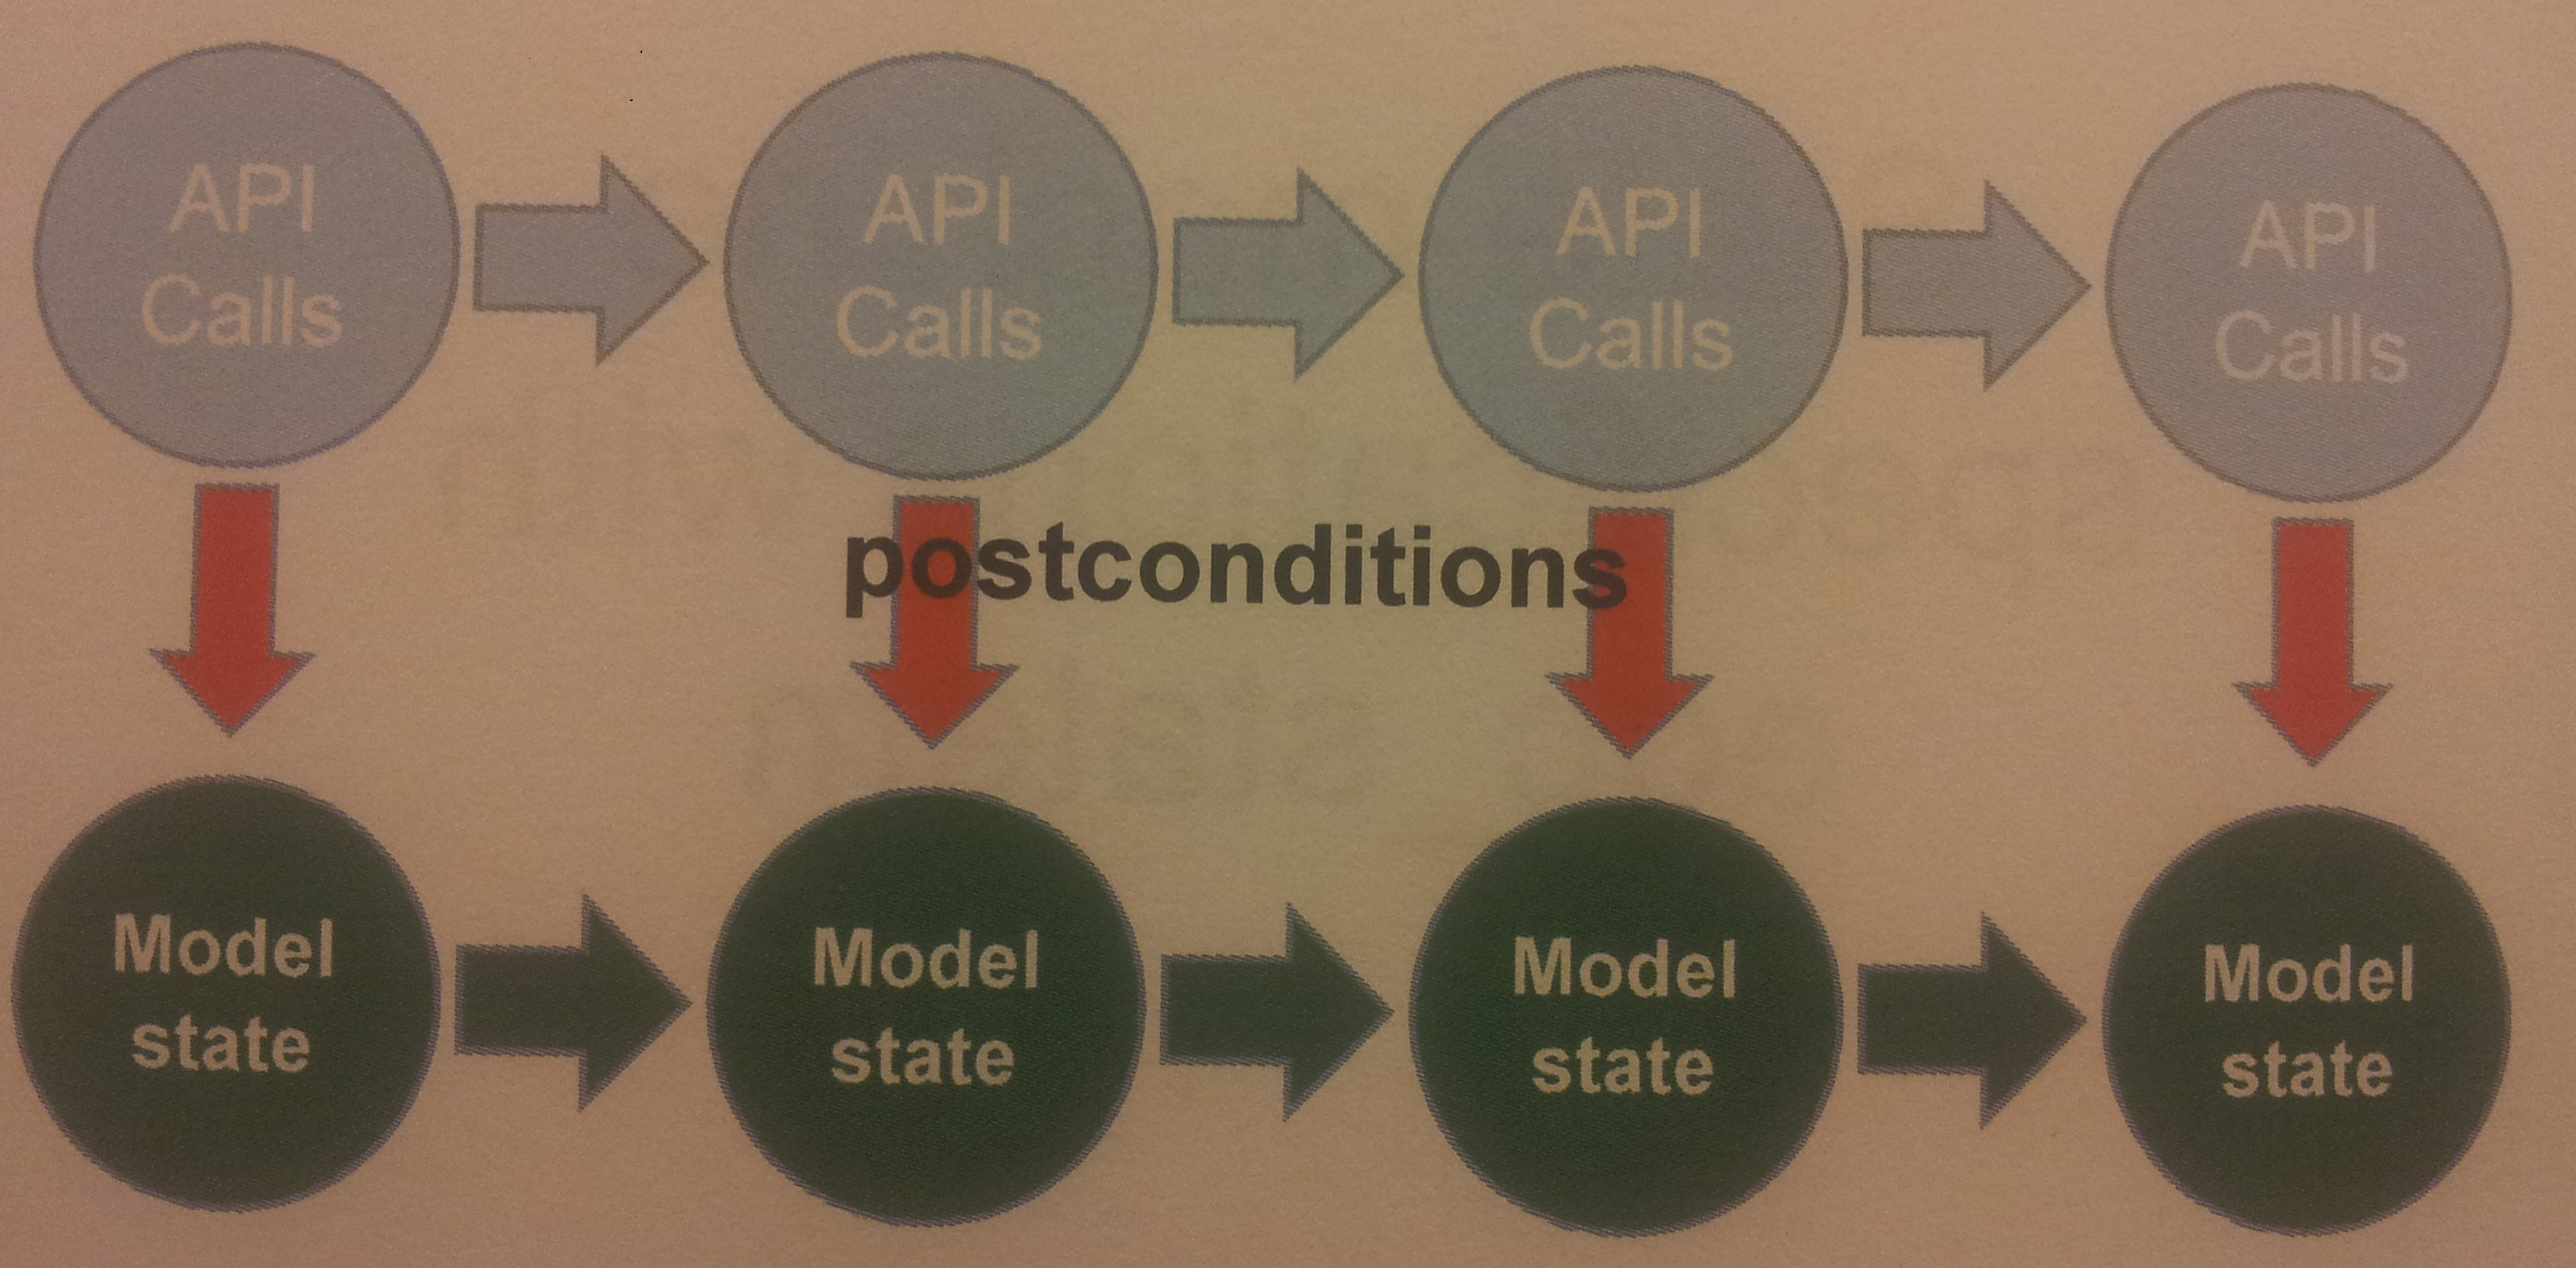
\includegraphics[keepaspectratio, width=0.7\linewidth]{api_calls}
  }
\end{frame}

%------------------------------------------------
\subsection{Configurations}
%------------------------------------------------

\begin{frame}
  \frametitle{Configurations}
  Three different configurations\\
  \begin{description}
    \item[BSI] minimal configuration
    \item[Example] complex configuration
    \item[Freescale] realistic configuration
  \end{description}
\end{frame}

%----------------------------------------------
\subsection{Testing}
%----------------------------------------------
%----------------------------------------------
%\subsection{Negative testing}
%----------------------------------------------

\begin{frame}
  \frametitle{Testing}
  \begin{block}{Positive testing}
    \begin{itemize}
      \item No absorbing state
      \item Correct arguments
      \item Correct command sequences
    \end{itemize}
  \end{block}
  \begin{block}{Negative testing}
    \begin{itemize}
      \item Invalid arguments
      \item Null pointers
      \item Absorbing state
    \end{itemize}
  \end{block}
\end{frame}

%================================================
\section{Bugs}
%================================================
%================================================
% \section{How to handle bugs}
%================================================
\begin{frame}
  \frametitle{Bugs}
  \begin{itemize}
    \item Report bug
    % \item[+] Not our job to correct the code
    % \item[-] Unknown time delay, probably weeks...
    % \item Skip the function with the bug
    % \item[+] We can continue testing
    % \item[-] After finding some bugs, we don't have anything to test
    % at all
    \item ``Fix'' the model
    % \item[+] We can continue testing
    % \item[-] Can't test c-code from another configuration or updated
    % version etc.
    \item Fix C-code
    % \item[+] We can continue testing
    % \item[-] Time consuming; need to get knowledge of the structure
    % etc.
    % \item Mocking function with bug
    % \item[+] We can continue testing
    % \item[-] Need to make a model for how it should work. The pitfall
    %   is if we implement the mocked function after the state machine.
  \end{itemize}
\end{frame}

%================================================
% \section{The bugs have we found}
%================================================
%------------------------------------------------
% \subsection{C-code}
%------------------------------------------------

\begin{frame}
  \frametitle{Bugs we found}
  \begin{block}{C code}
    Alot
  \end{block}

  \begin{block}{Generated C code}
    Some
  \end{block}

  \begin{block}{AUTOSAR complications}
    \begin{itemize}
      \item ambiguous meaning
      \item conflicting requirements
      \item omitted requirements/explanations
      \item spelling of configuration parameters
      \item references
    \end{itemize}
  \end{block}

  % \begin{tabular}{l l}
  %   Requirement & Our classification\\\hline
  %   WDGM286 & Medium\\
  %   WDGM077 & Low-Medium\footnote{\label{footnot:ett} Together their classification is Medium-High}\\
  %   WDGM117 & Low-Medium$^{\ref{footnot:ett}}$ \\
  %   WDGM215 & Low-Medium$^{\ref{footnot:ett}}$ \\
  %   WDGM216 & Low-Medium$^{\ref{footnot:ett}}$ \\
  %   WDGM219 & Low-Medium$^{\ref{footnot:ett}}$ \\
  %   WDGM220 & Low-Medium$^{\ref{footnot:ett}}$ \\
  %   WDGM182 & High\\
  %   7.2.3.2 & Medium\footnote{\label{footnot:tva} Together with WDGM252 and WDGM274
  %     this could be dangerous}\\
  %   WDGM255 & Low\\
  %   fig. 4  & Low
  % \end{tabular}
\end{frame}

%------------------------------------------------
%\subsection{Generated C-code}
%------------------------------------------------

% \begin{frame}
%   \frametitle{Generated C-code and include-files}
%   \begin{tabular}{l l}
%     Requirement & Our classification\\\hline
%     p. 27       & Low\\
%     fig. 4      & Low\\
%   \end{tabular}
% \end{frame}

%------------------------------------------------
%\subsection{AUTOSAR}
%------------------------------------------------

% \begin{frame}
%   \frametitle{AUTOSAR}
%   AUTOSAR complications
%   \begin{itemize}
%     \item ambiguous meaning
%     \item conflicting requirements
%     \item omitted requirements/explanations
%     \item spelling of configuration parameters
%     \item references
%   \end{itemize}
% \end{frame}

%================================================
\section{Coverage \& Statistics}
%================================================
%------------------------------------------------
%\subsection{Coverage}
%------------------------------------------------

\begin{frame}[fragile]
  \frametitle{Coverage \& Statistics}
  \begin{block}{Coverage}
    \begin{itemize}
      \item Line coverage of Erlang code (97.38\%)
      \item Function coverage of the C code (100\%)
      \item Condition/Decision coverage of C code (81\%)
      \item State space coverage (100\% of valid transitions, 0\% of invalid transitions)
    \end{itemize}
  \end{block}
  \begin{block}{Statistics}
    \begin{itemize}
      \item Generated command sequences of up to 120 commands (really no limit)
      \item 95\% starts with the command \verb!WdgM_Init!
    \end{itemize}
  \end{block}
\end{frame}

%================================================
\section{Functional Safety}
%================================================
\begin{frame}[fragile]
  \frametitle{Development Error Detection}
  Dangerous configuration parameter.
\end{frame}

%================================================
\section{Future work}
%================================================
\begin{frame}[fragile]
  \frametitle{Future work}
  Integration testing.

  More configurations = better test results.
\end{frame}

%================================================
\section{Conclusions}
%================================================
\begin{frame}
  \frametitle{Conclusions}
  QuickCheck and functional safety.

  AUTOSAR as a standard.

  Complexity of configurations.

  Measurements of state space, and code coverages.
\end{frame}

%================================================
\section{Questions}
%================================================
\begin{frame}
  \Huge{\centerline{Questions?}}
\end{frame}

\end{document}
